\documentclass[paper=a4, fontsize=11pt]{article} % A4 paper and 11pt font size
\usepackage[a4paper, margin=1.3in]{geometry}
% ---- Entrada y salida de texto -----

\usepackage[T1]{fontenc} % Use 8-bit encoding that has 256 glyphs
\usepackage[utf8]{inputenc}
% \usepackage[light,math]{iwona}

\usepackage{fancyhdr}
\usepackage{fancybox}
\usepackage{pseudocode}


% ---- Idioma --------

\usepackage[spanish, es-tabla]{babel} % Selecciona el español para palabras introducidas automáticamente, p.ej. "septiembre" en la fecha y especifica que se use la palabra Tabla en vez de Cuadro

% ---- Otros paquetes ----

\usepackage{amsmath,amsfonts,amsthm} % Math packages
\usepackage{graphics,graphicx, floatrow} %para incluir imágenes y notas en las imágenes
\usepackage{graphics,graphicx, float} %para incluir imágenes y colocarlas
\usepackage{enumerate}
\usepackage{subfigure}
% \makesavenoteenv{tabular}
% \makesavenoteenv{table}
% Para hacer tablas comlejas
%\usepackage{multirow}
%\usepackage{threeparttable}
\usepackage{sectsty} % Allows customizing section commands
\allsectionsfont{\centering \scshape} % Make all sections centered, the default font and small caps

\usepackage{fancyhdr} % Custom headers and footers
\usepackage[usenames, dvipsnames]{color}
\usepackage{colortbl}
% \usepackage{minted}
\usepackage{xcolor}
\usepackage{url}
\usepackage{cancel}

% \newmintedfile[mycpp]{c++}{
%     linenos,
%     numbersep=5pt,
%     gobble=0,
%     frame=lines,
%     framesep=2mm,
% }

% \newmintedfile[myc]{c}{
%     linenos,
%     numbersep=5pt,
%     gobble=0,
%     frame=lines,
%     framesep=2mm,
% }

% \newmintedfile[mypython]{python}{
%     linenos,
%     numbersep=5pt,
%     gobble=0,
%     frame=lines,
%     framesep=2mm,
% }

\usepackage{cite}

\usepackage[bookmarks=true,
    bookmarksnumbered=false, % true means bookmarks in
             % left window are numbered
    bookmarksopen=false,   % true means only level 1
             % are displayed.
    colorlinks=true,
    urlcolor=webblue,
    citecolor=webred,
    linkcolor=webblue]{hyperref}
\definecolor{webgreen}{rgb}{0, 0.5, 0} % less intense green
\definecolor{webblue}{rgb}{0, 0, 0.5}  % less intense blue
\definecolor{webred}{rgb}{0.5, 0, 0} % less intense red

%% Define a new 'leo' style for the package that will use a smaller font.
\makeatletter
\def\url@leostyle{%
  \@ifundefined{selectfont}{\def\UrlFont{\sf}}{\def\UrlFont{\small\ttfamily}}}
\makeatother
%% Now actually use the newly defined style.
\urlstyle{leo}

\pagestyle{fancyplain} % Makes all pages in the document conform to the custom headers and footers
\fancyhead{} % No page header - if you want one, create it in the same way as the footers below
\fancyfoot[L]{} % Empty left footer
\fancyfoot[C]{} % Empty center footer
\fancyfoot[R]{\thepage} % Page numbering for right footer
\renewcommand{\headrulewidth}{0pt} % Remove header underlines
\renewcommand{\footrulewidth}{0pt} % Remove footer underlines
\setlength{\headheight}{13.6pt} % Customize the height of the header

\numberwithin{equation}{section} % Number equations within sections (i.e. 1.1, 1.2, 2.1, 2.2 instead of 1, 2, 3, 4)
\numberwithin{figure}{section} % Number figures within sections (i.e. 1.1, 1.2, 2.1, 2.2 instead of 1, 2, 3, 4)
\numberwithin{table}{section} % Number tables within sections (i.e. 1.1, 1.2, 2.1, 2.2 instead of 1, 2, 3, 4)

\setlength\parindent{0pt} % Removes all indentation from paragraphs - comment this line for an assignment with lots of text

\newcommand{\horrule}[1]{\rule{\linewidth}{#1}} % Create horizontal rule command with 1 argument of height

%%%%% Para cambiar el tipo de letra en el título de la sección %%%%%%%%%%%
% \usepackage{sectsty}
% \chapterfont{\fontfamily{pag}\selectfont} %% for chapter if you want
% \sectionfont{\fontfamily{pag}\selectfont}
% \subsectionfont{\fontfamily{pag}\selectfont}
% \subsubsectionfont{\fontfamily{pag}\selectfont}

%----------------------------------------------------------------------------------------
% TÍTULO Y DATOS DEL ALUMNO
%----------------------------------------------------------------------------------------

\title{
\normalfont \normalsize
\textsc{{\bf Visión por Computador (2016-2017)} \\ Grado en Ingeniería Informática \\ Universidad de Granada} \\ [25pt] % Your university, school and/or department name(s)
\horrule{0.5pt} \\[0.4cm] % Thin top horizontal rule
\huge Proyecto Final\\Reconocimiento de Flores\\% The assignment title
\horrule{2pt} \\[0.5cm] % Thick bottom horizontal rule
}

\author{Marta Gómez Macías\\Correo: mgmacias95@correo.ugr.es\\
Braulio Vargas López\\Correo: brauliovarlop@correo.ugr.es} % Nombre y apellidos

\date{\normalsize\today} % Incluye la fecha actual

%----------------------------------------------------------------------------------------
% DOCUMENTO
%----------------------------------------------------------------------------------------

\begin{document}

\maketitle % Muestra el Título
\pagenumbering{gobble}
\newpage %inserta un salto de página

\tableofcontents % para generar el índice de contenidos
\newpage
\pagenumbering{arabic}

\section{Definición del problema}

El problema elegido consiste en extraer una serie de características del conjunto de imágenes para ser capaces de reconocer la especie de flor que es de las 17 especies posibles, mediante una imagen. Este problema consta de varias partes:

\begin{enumerate}
    \item \textbf{Extracción de las características principales de la imagen}.
    \item \textbf{Entrenar un algoritmo de aprendizaje a partir de las características extraídas}.
\end{enumerate}

Para esto, vamos a hacer uso de distintos descriptores, como son el descriptor \textit{HOG}, \textit{SIFT}, entre otros. Una vez tengamos los descriptores, utilizaremos la técnica \textit{Bag of Words} para obtener un descriptor que nos sirva para obtener un modelo de aprendizaje, capaz de clasificar las distintas clases de flores.

La técncia \textit{Bag Of Words} consiste en extraer una serie de características de las imágenes, conocidas como palabras. Cada imagen, tendrá una serie de palabras que la identifican y con estas palabras, podremos construir un vocabulario que almacena todas las palabras extraídas de todas las imágenes.

Con este vocabulario, podremos hacer un histograma que nos indica con qué fuerza vota o no una imagen a dichas palabras del vocabulario, con lo que obtendremos un vector de características de esa imagen, útil para el algoritmo de aprendizaje, y que no deja de tener relación con la propia imagen.

Este vocabulario lo podemos construir haciendo uso de técnicas que se centran en la geometría de la imagen y son invariantes a la escena, como son los descriptores de SIFT, SURF, etc. Pero, también es posible utilizar otro tipo de descritores como son el ya mencionado, HOG.

El descriptor HOG, conocido como \textit{\textbf{Histogram of Oriented Gradientes}} es muy utilizado para la detección de objetos. Este descriptor computa un histograma de valores donde se indican la frecuencia con la que se dan las direcciones de los gradientes en pequeñas divisiones de la imagen.

Hemos probado también a hacer un preprocesamiento de las imágenes convirtiéndolas al espacio de color HSV y simplificando los colores de las imágenes mediante la técnica \textbf{Color Quantization}\cite{cq}, para poder tener colores planos en la imagen. En la \hyperref[color]{Figura \ref*{color}} se ve una comparación entre una imagen sin ningún procesamiento previo y la misma imagen tras aplicar esta técnica. Esta técnica consiste en hacer grupos de colores mediante el algoritmo del \textit{Vecino más cercano} y sustituir todos los colores de un grupo por el más central. Así, se eliminan sombras y se simplifica la imagen para poder obtener mejores resultados.

\begin{figure}[!h]
  \centering
  \mbox{
    \subfigure[Una de las fotos del dataset sin ningún procesamiento] {
      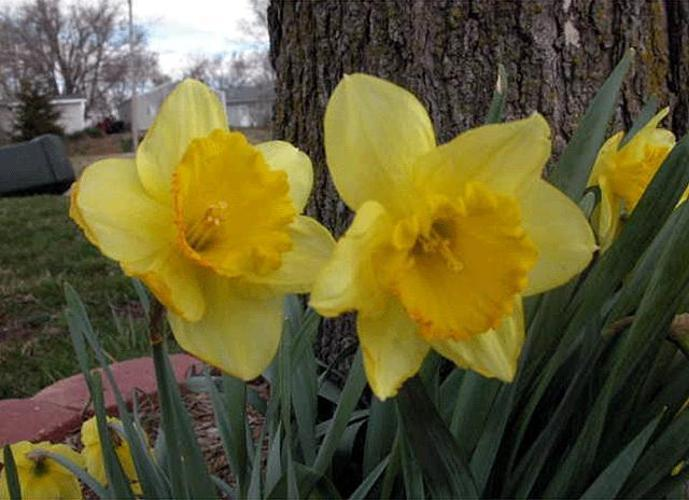
\includegraphics[width=0.5\textwidth]{../Dataset/image_0001}
      \label{imagen1}
    }
    \subfigure[La misma imagen, convertida al espacio de color HSV y con los colores simplificados] {
      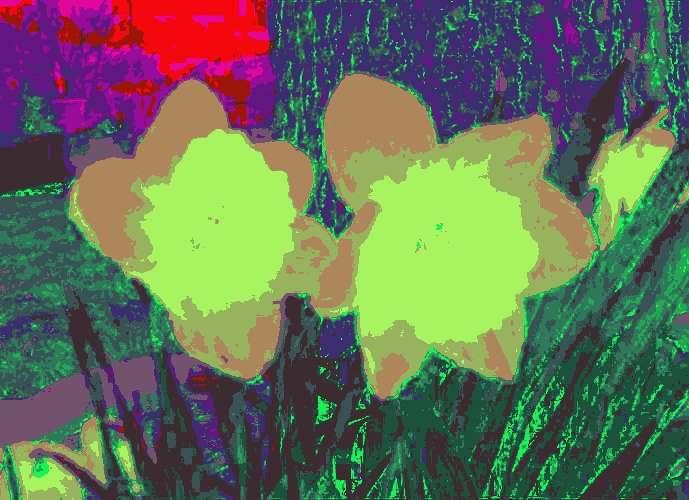
\includegraphics[width=0.5\textwidth]{../ColorQuantization/image_0001}
      \label{img1}
    }
  }
  \caption{Comparación de una foto con y sin el tratamiento de color que hemos hecho}
  \label{color}
\end{figure}

\section{Enfoque de la implementacion y eficiencia}

La implementación de este trabajo se ha realizado entera en Python, usando la librería OpenCV para la parte de visión por computador, y la librería \textit{scikit-learn}\cite{scikit-learn}.

\subsection{Extracción de las características principales de la imagen}

En primer lugar, hemos generado una función capaz de cargar todo el conjunto de datos de la carpeta \textit{Dataset} en memoria para poder comenzar a trabajar con las imágenes.

A continuación, para poder extraer las características de una imagen, primero hemos implementado una función que calcula varios tipos de descriptores de una imagen, según el tipo de detector que queramos usar. Según el tipo de descriptor, generará un detector que irá construyendo un vocabulario, a partir de los \textit{KeyPoints} detectados y su descriptor.
Este vocabulario se inicializa como un \texttt{BOWKMeansTrainer} y con la función \texttt{add} vamos añadiendo los descriptores obtenidos.

\subsection{Clusterizar los descriptores obtenidos}

Para obtener los clusters, al haber creado el vocabulario con \texttt{BOWKMeansTrainer}, podemos usar la función cluster para realizar el clustering con K-Medias y así obtener el vocabulario clusterizado, listo para obtener los descriptores de cada imagen.
Esta función de OpenCV, ya implementa el método de clustering utilizando multiprocesamiento en paralelo, para aumentar la eficiencia del algoritmo.

\subsection{Obtener los histogramas de cada imagen}

Una vez construida la bolsa de palabras, tenemos ver con qué fuerza vota cada una de las imágenes para las distintas palabras que hemos extraído. Para ello, utilizaremos la función de OpenCV \texttt{BOWImgDescriptorExtractor}, que necesita un detector de puntos, que crearemos del mismo tipo que se usó para la construcción del vocabulario, y un \textit{matcher}. En este caso, usaremos un \textit{matcher} basado en fuerza fuerza bruta.
Con todo esto, podremos calcular el histograma para cada imagen y obtener el descriptor para cada una de ellas, haciendo uso de la función de OpenCV compute que utiliza la imagen y el detector para obtener los \textit{KeyPoints} y computar el histograma.

\subsection{Pruebas}

En esta última parte, comprobaremos cómo de efectivos han sido los datos extraídos. Para ello, se han usado dos algoritmos de aprendizaje automático, dos \textit{Support Vector Machine} (SVM), uno siguiendo el método \textit{one-vs-all} y otro, el método \textit{one-vs-one}, y dos \textit{Random Forest}, uno aplicando \textit{bootsting} y otro sin aplicarlo. La ejecución de un modelo u otro no requiere más de 5 minutos, gracias a que cada algoritmo se ejecuta de forma paralela.

Para comprobar la eficacia de los modelos, usaremos validación cruzada al tener un conjunto de datos pequeño ($n=1360$).

También se han realizado pruebas para ver cómo la decisión de tomar un descriptor u otro afecta a la calidad del clasificador.

\section{Experimentación}

El conjunto de datos dispone un total de 1360 imágenes de tamaños más o menos similares, generalmente de $600\times500$ aproximadamente, con la flor centrada en la imagen. Las principales dificultades que tienen las imágenes, es que las flores aparecen en las imágenes, no son tomadas desde el mismo ángulo, sino que aparecen imágenes de flores pertenecientes a la misma especie, tomadas desde distintos ángulos, y en ocasiones, con distinta luz, además de las propias diferencias que pueden existir entre flores distintos individuos de la misma especie.

Hemos experimentado con tres tipos de datos distintos: con las imágenes sin ningún procesamiento, con las imágenes procesadas con el algoritmo de \textit{Color Quantization} y con ambas a la vez.


\subsection{Imágenes sin procesamiento previo}
Para empezar, decidimos usar el descriptor de SIFT para extraer los \textit{KeyPoints} de cada imagen y sus respectivos descriptores para poder crear diccionario de palabras.

Este diccionario se ha realizado usando el algoritmo \textit{K-Means} para el clustering, realizando distintas ejecuciones cambiando el tamaño de $k$ en el intervalo $[20,1000]$. El tiempo de ejecución del clustering depende del tamaño, pero para $k=1000$ supone un tiempo de 30 minutos aproximadamente.

Para tamaño $k=20$ en clustering, tenemos las siguientes tasas de acierto en la \hyperref[res1]{Tabla \ref*{res1}}:

\begin{table}[H]
  \begin{tabular}{l|r}
    \textbf{Algoritmo} & \textbf{Tasa de acierto} \\
    \hline
    \textit{SVM one-vs-all} & $\qquad$ 0.63 \\
    \textit{SVM one-vs-one} & $\qquad$ 0.63 \\
    \textit{RF con bootsting} & $\qquad$ 0.65 \\
    \textit{RF sin bootsting} & $\qquad$ 0.59 \\
  \end{tabular}
  \label{res1}
  \caption{Tasa de aciertos de los algoritmos usando sólo la geometría de la imagen.}
\end{table}

\subsection{Imágenes con procesamiento \textit{Color Quantization}}

\begin{table}[H]
  \begin{tabular}{l|r}
    \textbf{Algoritmo} & \textbf{Tasa de acierto} \\
    \hline
    \textit{SVM one-vs-all} & $\qquad$ 0.47 \\
    \textit{SVM one-vs-one} & $\qquad$ 0.47 \\
    \textit{RF con bootsting} & $\qquad$ 0.47 \\
    \textit{RF sin bootsting} & $\qquad$ 0.47 \\
  \end{tabular}
  \label{res2}
  \caption{Tasa de aciertos de los algoritmos usando imágenes con \textit{Color Quantization}.}
\end{table}

\subsection{Usando información de los dos experimentos anteriores}

\begin{table}[H]
  \begin{tabular}{l|r}
    \textbf{Algoritmo} & \textbf{Tasa de acierto} \\
    \hline
    \textit{SVM one-vs-all} & $\qquad$ 0.63 \\
    \textit{SVM one-vs-one} & $\qquad$ 0.63 \\
    \textit{RF con bootsting} & $\qquad$ 0.65 \\
    \textit{RF sin bootsting} & $\qquad$ 0.65 \\
  \end{tabular}
  \label{res2}
  \caption{Tasa de aciertos de los algoritmos usando la información de los dos experimentos anteriores.}
\end{table}

\bibliography{citations} %archivo citas.bib que contiene las entradas 
\bibliographystyle{plain} % hay varias formas de citar

\end{document}